\chapter{Application à l'étude de la dégradation du D-Apiose}

Le D-Apiose est un sucre de type pentose, principalement retrouvé dans la paroi cellulaire des plantes vasculaires, mais également présent en tant que métabolite secondaire \cite{picmanova_apiose_2016}. Chez les bactéries, plusieurs voies de dégradation du D-Apiose ont été identifiées \cite{carter_functional_2018}. Parmi celles-ci, la voie de la transcétolase non oxydante (\autoref{fig:apiosePathway}) constitue un mécanisme clé. Cette voie permet la conversion du D-Apiose en D-xylulose 5-phosphate, un métabolite intermédiaire central impliqué dans de nombreuses voies métaboliques essentielles. La voie de la transcétolase non oxydante a été détectée chez diverses bactéries du sol, notamment \textit{Actinobacillus succinogenes} et \textit{Bacteroides vulgatus}, ainsi que chez plusieurs espèces du genre \textit{Pectobacterium}.

En collaboration avec Guilhem Royer (AP-HP) et Erick Denamur (IAME), le LABGeM a identifié une voie alternative chez \textit{Escherichia coli}, où l'isomérase de la première réaction est remplacée par une succession de deux oxydoréductases. Cette voie a été initialement identifiée spécifiquement dans les \textit{Sequence Types} (ST) 131 et 14 de \textit{E. coli}, des souches pathogènes connues pour leur multirésistance aux antibiotiques et leur implication dans les bactériémies\footnote{Infection bactérienne présente dans le sang.} \cite{schembri_molecular_2015,de_korne-elenbaas_putative_2023}. Ces souches colonisent principalement le tube digestif, où la capacité à dégrader le D-Apiose pourrait conférer un avantage sélectif, améliorant ainsi le \textit{fitness} de ces pathogènes.

Dans ce cadre, j’ai contribué au projet en explorant les pangénomes afin d’identifier le contexte génomique associé à la fois à la voie classique (transcétolase non oxydante) et à la voie alternative de dégradation du D-Apiose.

\begin{figure}[htbp]
    \centering
    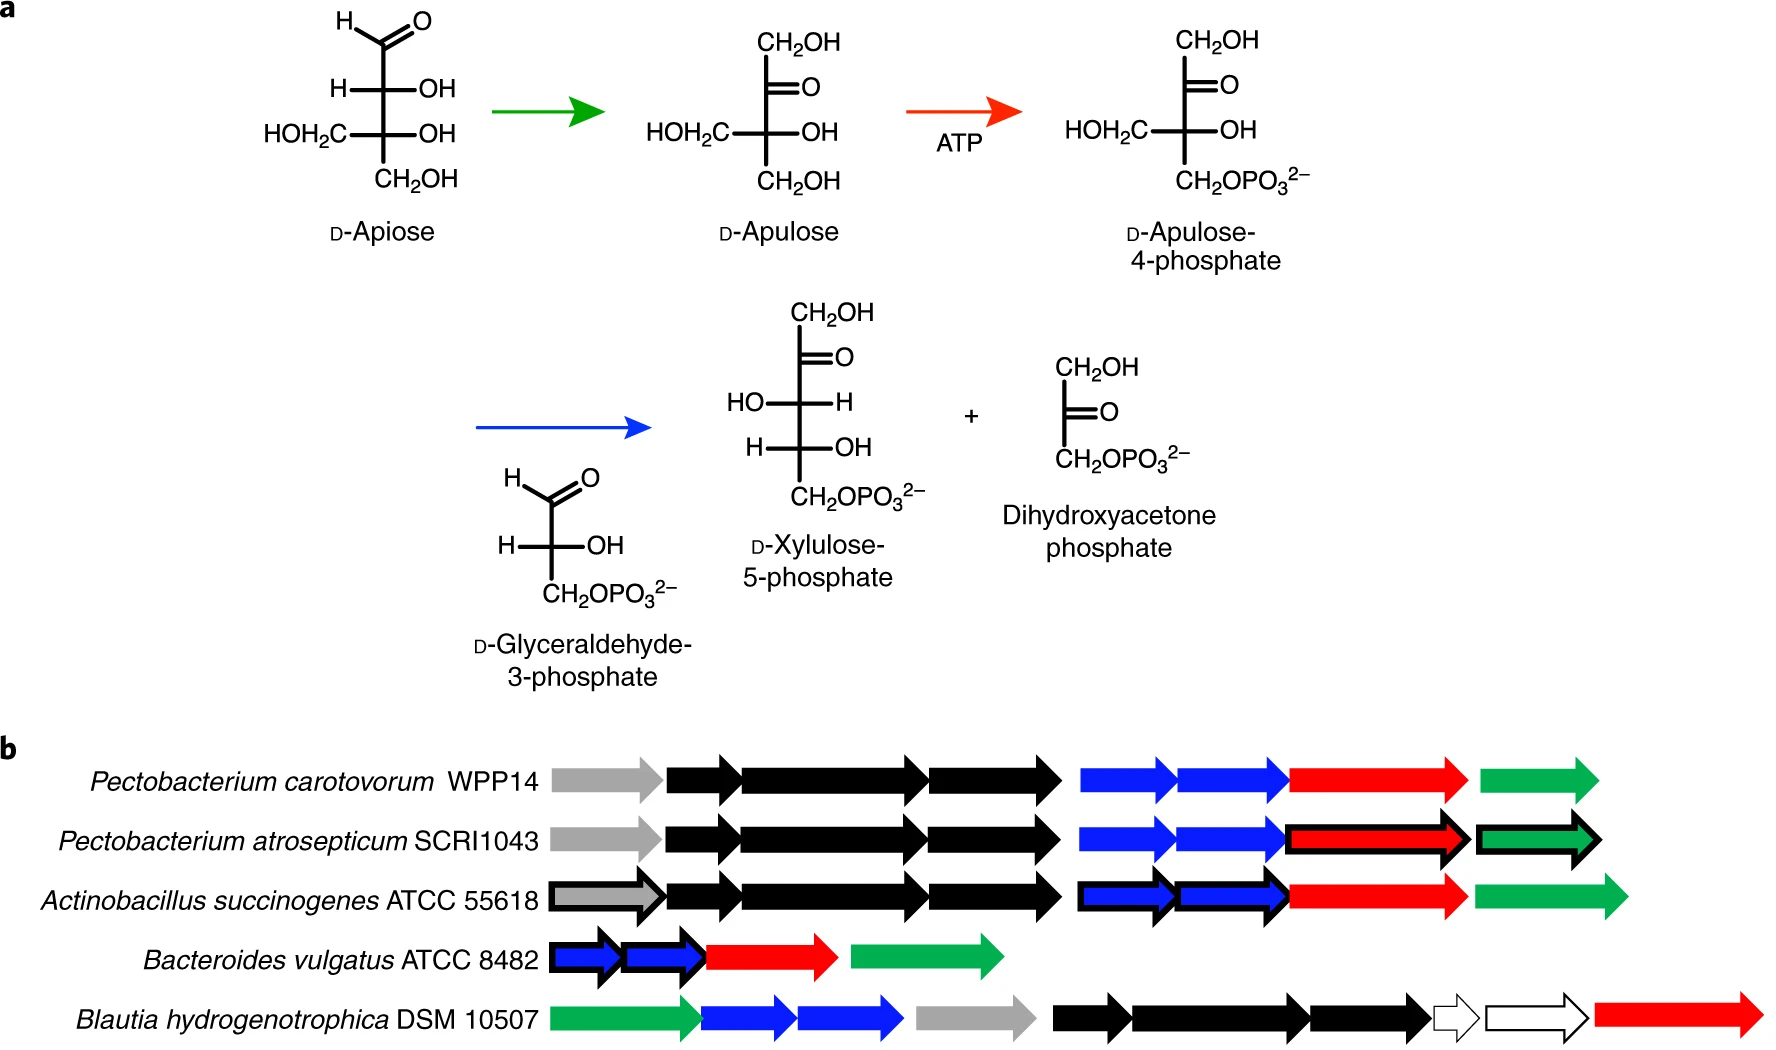
\includegraphics[width=0.75\linewidth]{images/ApiosePathway.png}
    \caption[Voie de dégradation du D-Apiose par la transcétolase non oxydante]{\textbf{Voie de dégradation du D-Apiose par la transcétolase non oxydante.} (a) Métabolites et réactions de la voie. La première réaction (en vert) correspond à l'isomérisation du D-Apiose en D-Apulose, catalysée par la D-Apiose isomérase. Le D-Apulose est ensuite phosphorylé en D-Apulose 4-phosphate (en rouge) par l’action d’une kinase. Enfin, la dernière transformation (en bleu) est catalysée par la transcétolase, qui permet la production du D-xylulose 5-phosphate. (b) Contexte génomique de la voie de dégradation chez cinq espèces bactériennes. Les gènes impliqués sont représentés par des flèches colorées, dont la couleur correspond à l’enzyme codée. Les gènes gris codent des SBP (protéines de liaison spécifiques) impliqués dans la reconnaissance du D-Apiose, tandis que les gènes noirs codent des composants d’un système de transport ABC. Extrait de \cite{carter_functional_2018}.}
    \label{fig:apiosePathway}
\end{figure}

\section{Recherche du contexte génomique chez les procaryotes}

Nous avons commencé par rechercher la voie de dégradation du D-Apiose, à la fois sous sa forme classique (transcétolase non oxydante) et sous sa forme alternative, dans les espèces procaryotes. Pour cela, nous avons analysé le contexte génomique associé aux six protéines clés impliquées dans ces voies. Ces protéines incluent : 3 enzymes communes aux deux voies, les deux sous-unités de la transcétolase et la kinase; une enzyme spécifique à la voie classique l'isomérase; 2 enzymes spécifiques à la voie alternative, les oxydoréductases.

L’analyse du contexte génomique a été réalisée sur un ensemble de 1 429 pangénomes d’espèces, générés à l’aide de l’outil PPanGGOLiN\footnote{Les pangénomes ont été élaborés dans le cadre du projet PanGBank, visant à constituer une base de données de pangénomes d’espèces.}. Ces pangénomes ont été construits à partir de 152 717 génomes issus de la base de données RefSeq \cite{pruitt_ncbi_2007}, en utilisant la taxonomie GTDB \cite{parks_standardized_2018} pour organiser les génomes par espèce (version RefSeq/GTDB : 220).

\newpage

Le GC de dégradation du D-Apiose a été identifié dans 125 espèces, réparties sur 43 genres, 17 familles, 15 ordres, 7 classes et 4 phylums (\autoref{fig:PhyloTreeApiose}). Parmi ces familles, les \textbf{Enterobacteriaceae} sont les plus représentées (66 espèces), suivies des \textbf{Rhizobiaceae} (23 espèces) et des \textbf{Pseudomonadaceae} (12 espèces). Cette répartition suggère que la voie de dégradation du D-Apiose est relativement fréquente chez les bactéries.
L’analyse de la distribution des données au sein des partitions du pangénome révèle que cette voie est principalement associée à un contexte \textit{persistent}, avec 28 genres sur 43 présentant une majorité de familles classées dans cette même partition.

Parmi les contextes identifiés, seules 7 espèces présentent la voie classique de dégradation du D-Apiose. Six d’entre elles appartiennent au genre \textit{Pectobacterium} : \textit{P. atrosepticum}, \textit{P. brasiliense}, \textit{P. parmentieri}, \textit{P. carotovorum}, \textit{P. versatile} et \textit{P. polare}. La septième espèce, \textit{Novosphingobium capsulatum}, appartient à la famille des \textit{Sphingomonadaceae} et est représentée en bleu-vert clair sur la \autoref{fig:PhyloTreeApiose}. Contrairement aux espèces du genre \textit{Pectobacterium}, où le contexte génomique est retrouvé dans la partition \textit{persistent}, celui de \textit{N. capsulatum} se situe dans la partition \textit{shell}, ce qui pourrait suggérer un transfert horizontal de gènes (HGT) entre ces espèces.

Par ailleurs, 3 espèces possèdent une version hybride entre la voie classique et la voie alternative, caractérisée par la présence simultanée de l’isomérase et des 2 oxydoréductases. Deux d’entre elles appartiennent à la famille des \textit{Sphingomonadaceae}, à savoir \textit{Sphingobium yanoikuyae} et \textit{Sphingomonas koreensis}, tandis que la troisième, \textit{Klebsiella aerogenes}, appartient aux \textit{Enterobacteriaceae}. La présence de voies hybrides dans certaines espèces pourrait refléter une adaptation évolutive conférant une plus grande flexibilité métabolique en fonction des conditions environnementales.

\newpage

Enfin, des contextes partiels ont été détectés dans 13 espèces. Dix d’entre elles appartiennent à la famille des \textit{Enterobacteriaceae}, incluant \textit{Salmonella diarizonae}, \textit{Atlantibacter hermannii}, \textit{Yersinia enterocolitica}, \textit{Leclercia adecarboxylata}, \textit{Citrobacter youngae}, \textit{Yersinia bercovieri}, \textit{Kosakonia radicincitans}, \textit{Yersinia mollaretii}, \textit{Yersinia massiliensis} et \textit{Yersinia intermedia}. Deux autres espèces, \textit{Paracidovorax avenae} et \textit{Paracidovorax citrulli}, appartiennent à la famille des \textit{Burkholderiaceae}, tandis que \textit{Clostridioides difficile} représente la famille des \textit{Peptostreptococcaceae}. L’existence de ces contextes partiels pourrait être attribuée à la présence d’autres voies métaboliques alternatives, comme proposé par Carter \textit{et al.} \cite{carter_functional_2018}, ou être liée à la spécificité de l’isomérase au genre \textit{Pectobacterium}. L’analyse de la base de données UniProt \cite{the_uniprot_consortium_uniprot_2025} suggère en effet que cette enzyme présente une faible similarité avec celles d’autres organismes, ce qui pourrait expliquer l’absence apparente de la voie classique dans certaines espèces, alors qu’un homologue fonctionnel pourrait exister.

Des recherches complémentaires seront nécessaires pour mieux comprendre les implications fonctionnelles de ces variations et explorer les mécanismes évolutifs sous-jacents.

\begin{figure}[htbp] 
    \centering
    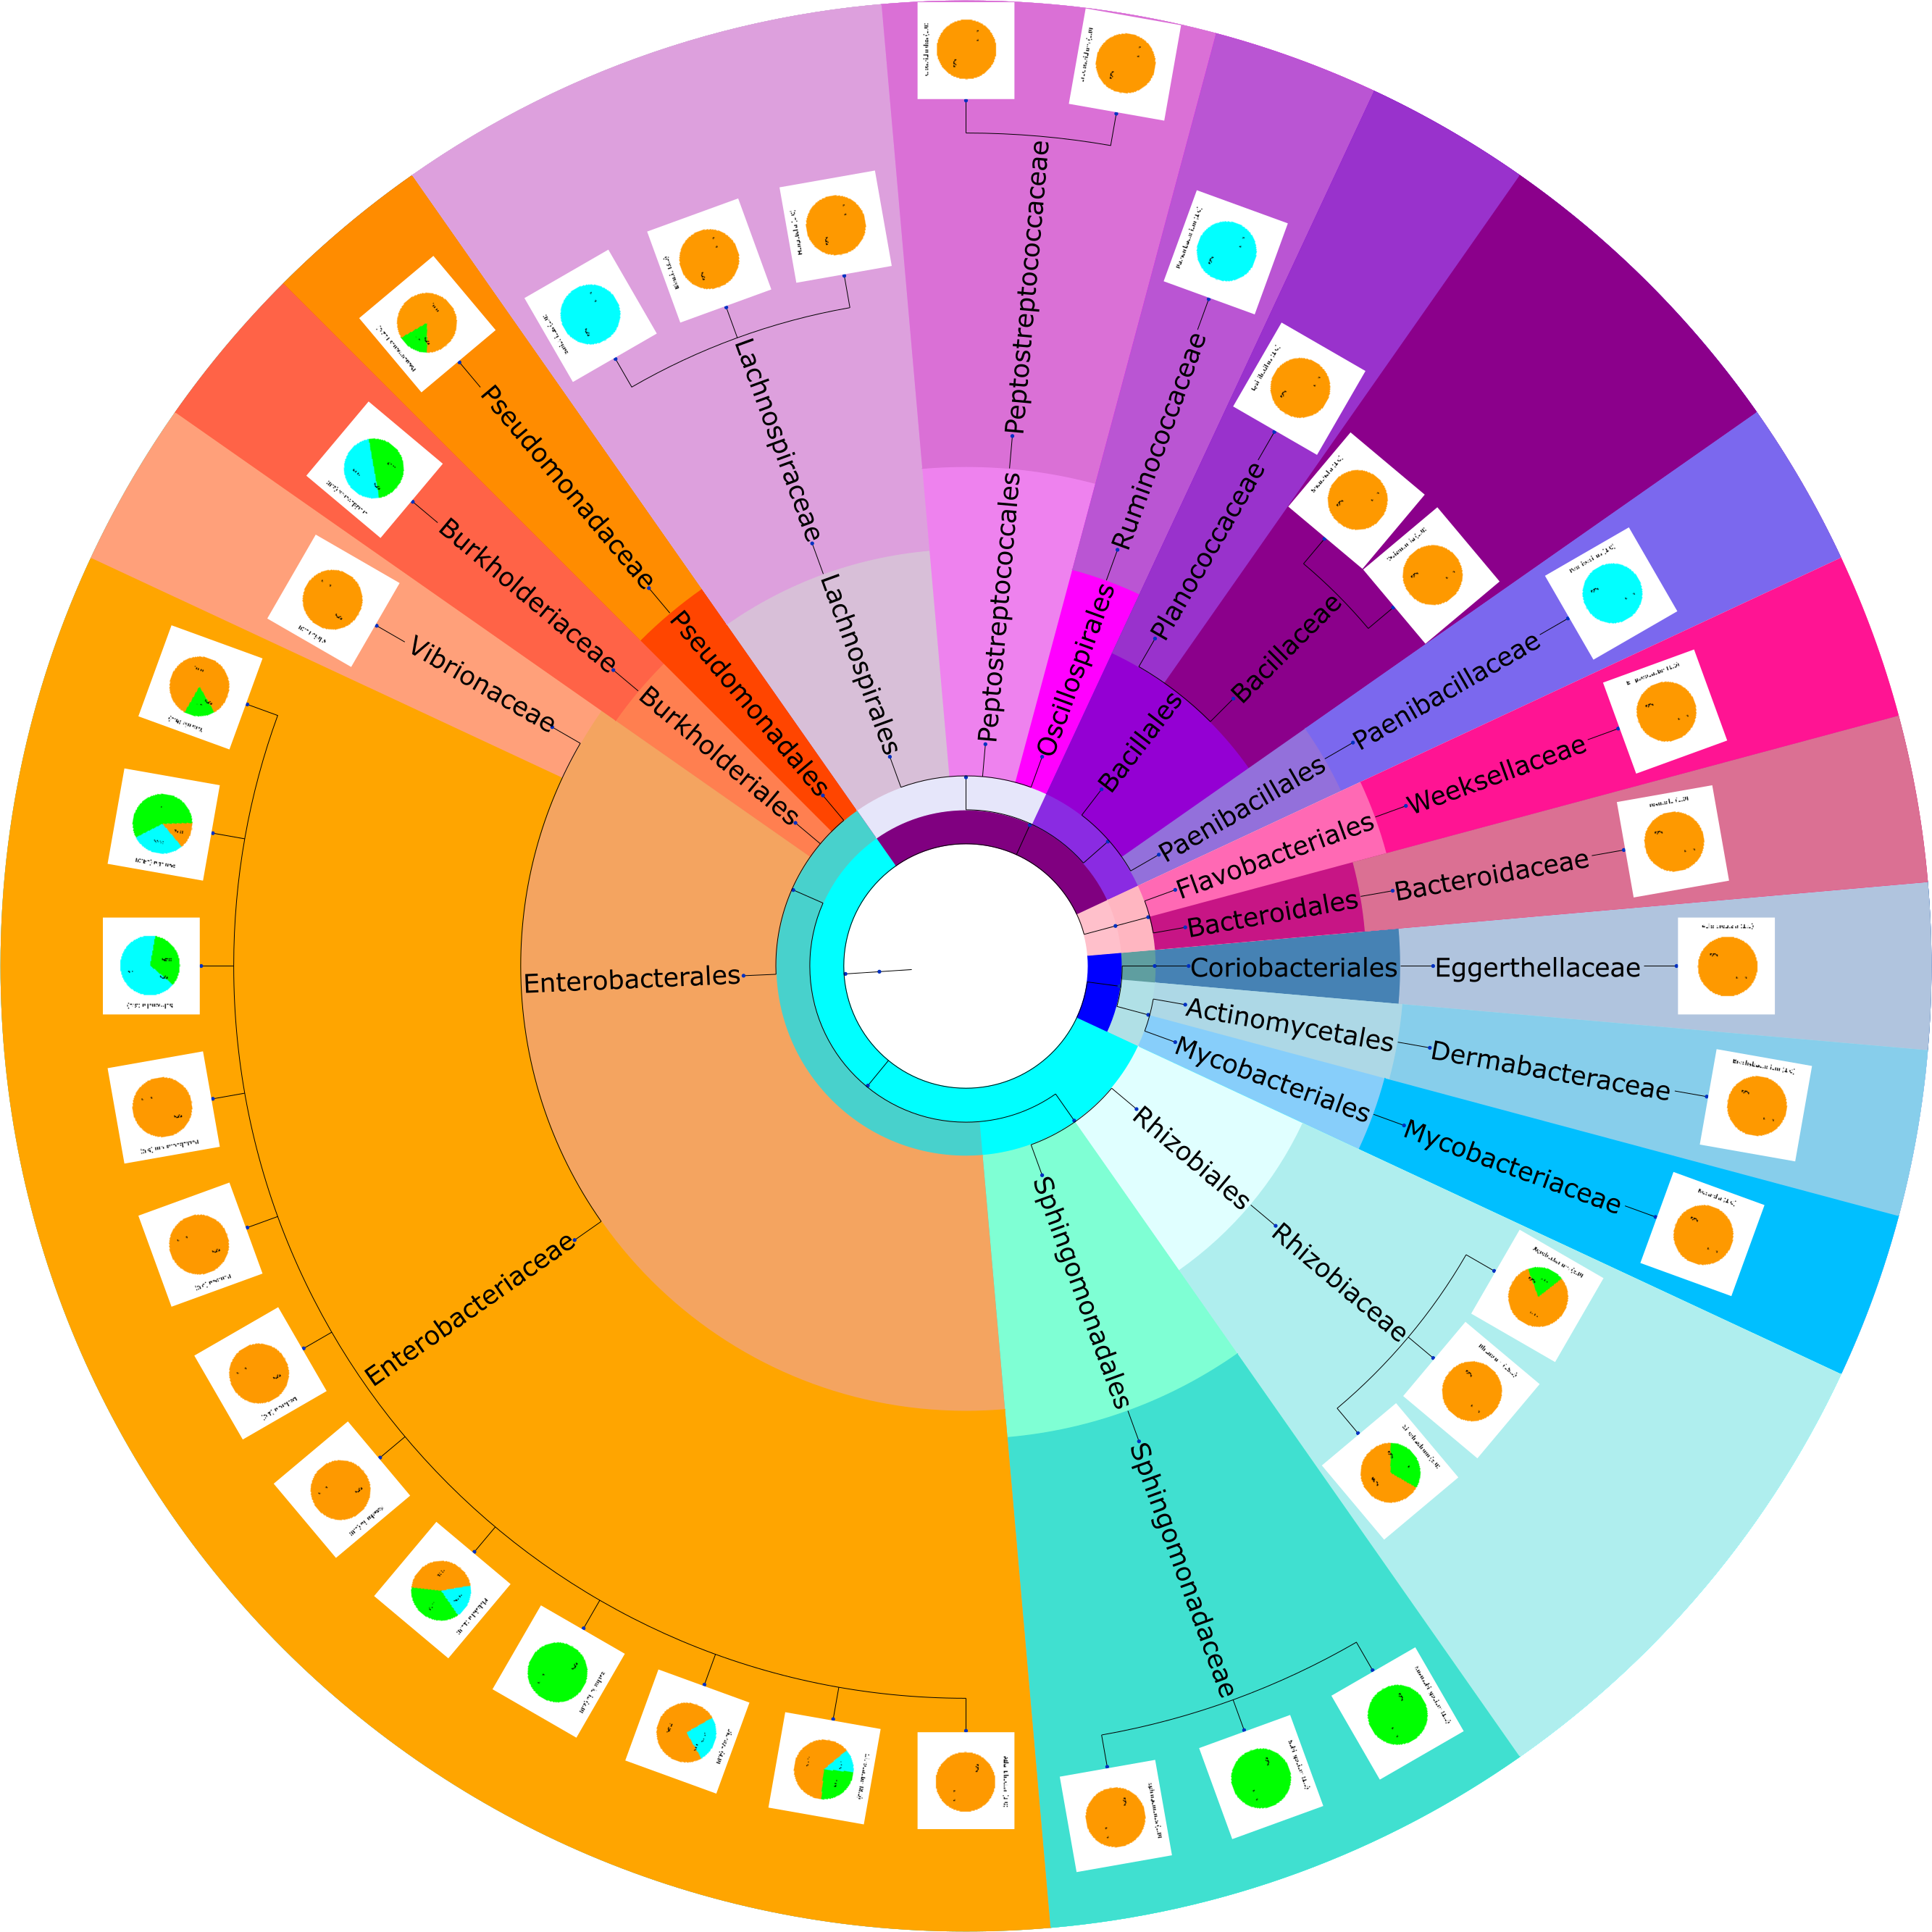
\includegraphics[width=\textwidth]{images/phylogenetic_tree_with_pies.png}
    \caption[Arbre taxonomique des procaryotes étiqueté par la présence de la voie de dégradation du D-Apiose]{\textbf{Arbre taxonomique des procaryotes étiqueté par la présence de la voie de dégradation du D-Apiose.} Si une branche existe alors un GC a été détecté sinon l'embranchement n'est pas créé. Les feuilles de l'arbre représente le niveau taxonomique du genre. Les \textit{pie chart} en bout de branche, représente la proportion de GC trouvé dans chaque partition du pangénome, indépendamment de la forme de la voie (classique, alternative, hybride ou partielle).} 
    \label{fig:PhyloTreeApiose}
\end{figure}

Nous avons ensuite centré notre étude sur la famille des Enterobacteriaceae, où la voie de dégradation du D-Apiose avait été initialement identifiée \cite{carter_functional_2018} et à laquelle \textit{Escherichia coli} appartient.
Comme l'illustre la \autoref{fig:clustermap_entero}, le contexte génomique est principalement retrouvé dans la partition \textit{persistent} (16 espèces), suivie de la partition \textit{shell} (8 espèces) et enfin de la partition \textit{cloud} (5 espèces). 
Ces espèces appartiennent à plusieurs genres bactériens, notamment Klebsiella, Citrobacter, Serratia et Escherichia. La majorité d’entre elles sont connues pour être des pathogènes humains, partageant un habitat commun : le tube digestif. D’un point de vue phylogénétique et taxonomique, ces bactéries sont étroitement apparentées à des espèces vivant dans les sols, où la dégradation du D-Apiose issu des plantes constitue un avantage sélectif. C’est notamment le cas de \textit{Pantoea vagans}, une espèce isolée à partir de feuilles d’eucalyptus \cite{brady_pantoea_2009}.
La présence de la voie alternative dans la partie variable du pangénome suggère une acquisition par transfert horizontal, au cours de laquelle cette nouvelle voie métabolique aurait été transférée des bactéries vivant dans les écosystèmes du sol vers celles colonisant le microbiote intestinal et gastrique.

\begin{figure}[htbp] 
    \centering
    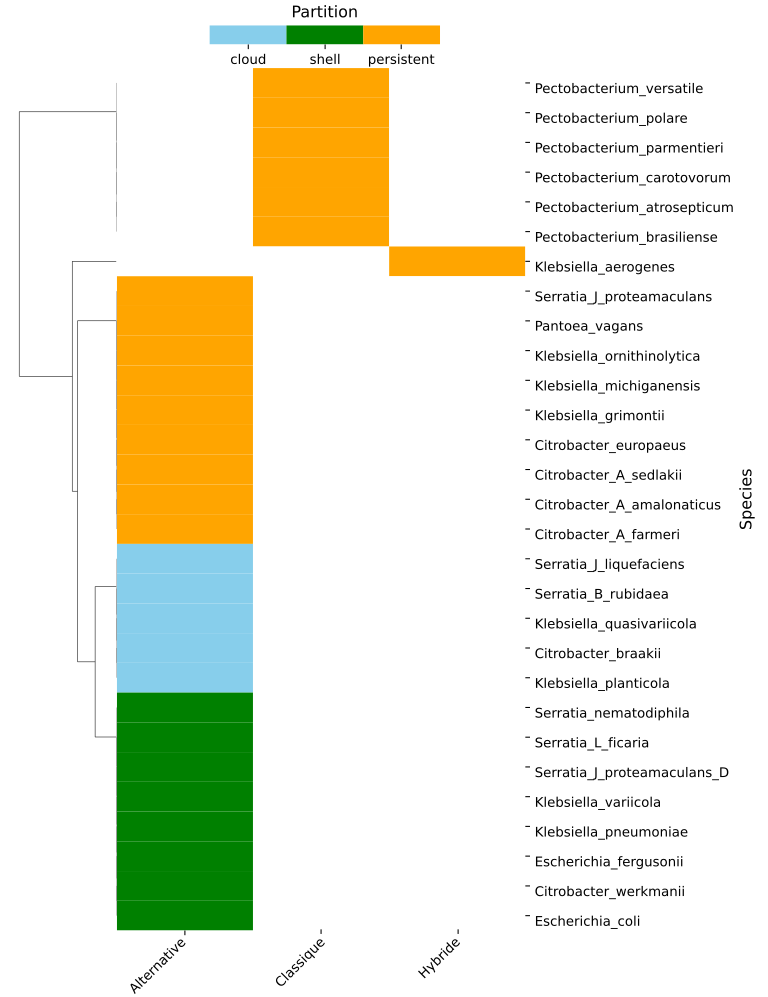
\includegraphics[width=.9\textwidth]{images/clustermap.png}
    \caption[Prédiction du contexte de dégradation du D-apiose dans les pangénomes des Enterobacteriaceae]{\textbf{Prédiction du contexte de dégradation du D-apiose dans les pangénomes des Enterobacteriaceae.}} 
    \label{fig:clustermap_entero}
\end{figure}

\newpage

\section{Analyse du pangénome de \textit{Escherichia coli}}

Nous avons ensuite recentré notre analyse sur l’espèce \textit{Escherichia coli}, dans laquelle la voie de dégradation du D-Apiose impliquant deux oxydoréductases avait été identifiée. Pour cela, nous avons exploité le pangénome construit précédemment à partir des bases de données RefSeq et GTDB \cite{pruitt_ncbi_2007,parks_standardized_2018}, dont la composition est indiquée dans le \autoref{tab:E_coli_pangenome}.

Le pangénome de \textit{E. coli} (\autoref{fig:pangenomeColi}) est majoritairement composé de familles variables (points bleus), avec des chemins \textit{persistent} (en orange) correspondant aux régions conservées. Au sein de ces chemins, on retrouve des régions variables, constituées d’éléments \textit{shell} (verts) et \textit{cloud}. Ces zones correspondent généralement à des spots d’insertion, où sont localisées des régions génomiques plastiques (RGPs). C’est dans ces régions variables que nous avons recherché le contexte génomique de la voie de dégradation du D-Apiose.


\begin{table}[htbp]
    \centering
    \begin{tabular}{|l|l|l|}
    \hline
    \textbf{Génomes} & \textbf{Gènes} & \textbf{Familles} \\
    \hline
    2006 & 9334727 & 57444 \\
    \hline
    \hline
    \textit{\textbf{Persistent}} & \textit{\textbf{Shell}} & \textit{\textbf{Cloud}} \\
    \hline
    3167 & 7960 & 46317\\
    \hline
    \hline
    \textbf{RGPs} & \textbf{Spots} & \textbf{Modules} \\
    \hline
    164573 & 1968 & 2089 \\
    \hline
    \end{tabular}
    \caption[Composition du pangénome de \textit{E. coli}]{\textbf{Composition du pangénome de \textit{E. coli}.} Le pangénome a été généré avec PPanGGOLiN et utilise les génomes de RefSeq \cite{pruitt_ncbi_2007} en suivant la taxonomie de GTDB \cite{parks_standardized_2018}}
    \label{tab:E_coli_pangenome}
\end{table}

\begin{figure}[htbp] 
    \centering
    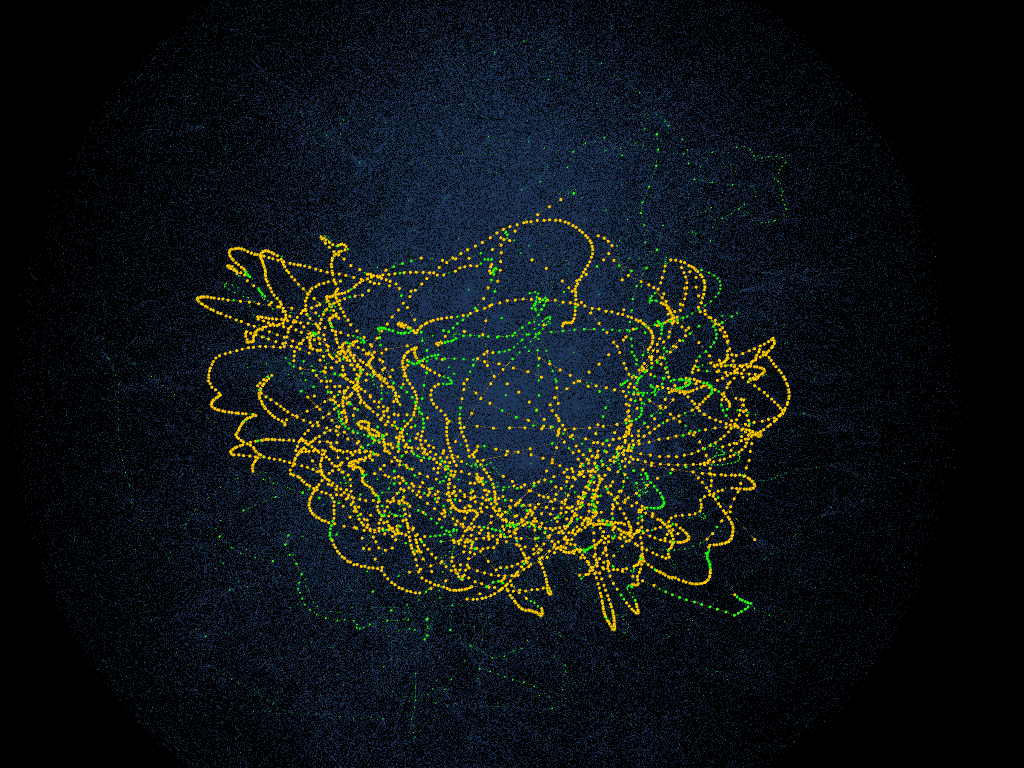
\includegraphics[width=.9\textwidth]{images/pangenome_ecoli.png}
    \caption[Graphe de pangénome de \textit{E. coli}]{\textbf{Graphe de pangénome de \textit{E. coli}.} Le graphe est visualisé avec Gephi \cite{bastian_gephi_2009}. L'algorithme de spatialisation utilisé est \textit{Force Atlas 2} avec une gravité forte et une échelle à 5 000.} 
    \label{fig:pangenomeColi}
\end{figure}


L’analyse a révélé que le contexte génomique associé à cette voie est localisé dans le spot 181 du pangénome (\autoref{fig:spot_apiose}). Ce spot d’insertion est identifié dans 62 génomes, chacun contenant une seule RGP. Parmi ces génomes, 31 possèdent le contexte de dégradation du D-Apiose. Comme illustré dans la \autoref{fig:spot_apiose}, ce contexte est également associé au module 752, qui est spécifique de la voie métabolique.

L’analyse de la composition en familles du module met également en évidence la conservation de plusieurs familles de gènes qui, bien que ne jouant pas un rôle enzymatique direct, sont essentielles au fonctionnement de la voie. On retrouve notamment plusieurs familles codant des transporteurs ABC, impliqués dans la capture et le transport du D-Apiose, ainsi qu’une lipoprotéine et un facteur de transcription. Ces éléments avaient déjà été partiellement décrits par Carter \textit{et al.} \cite{carter_functional_2018}. Toutefois, l’association systématique de ces gènes au contexte génomique prédit dans le pangénome confirme leur rôle étroit dans l’opérabilité de la voie métabolique.

\begin{figure}[htbp] 
    \centering
    \subfloat[]{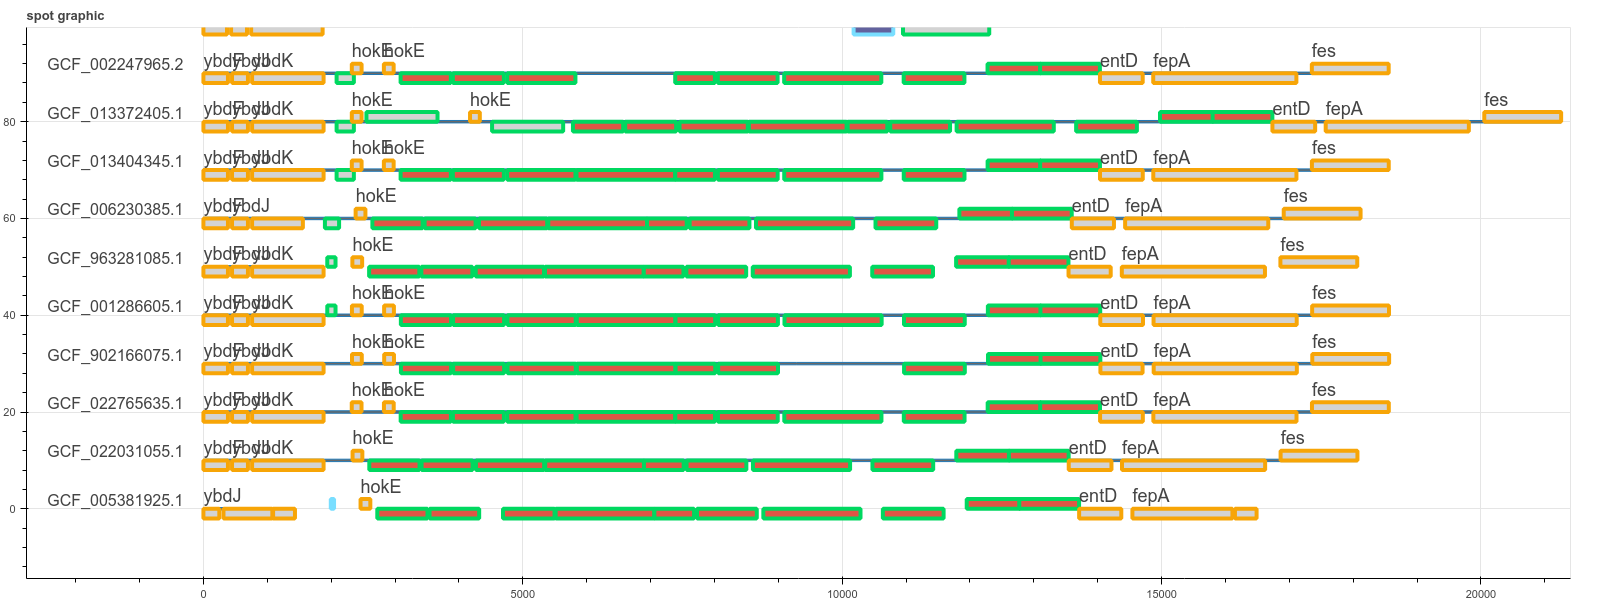
\includegraphics[width=0.6\textheight, angle=-90]{images/spot_181_module.png}}
    \hspace{1cm}
    \subfloat[]{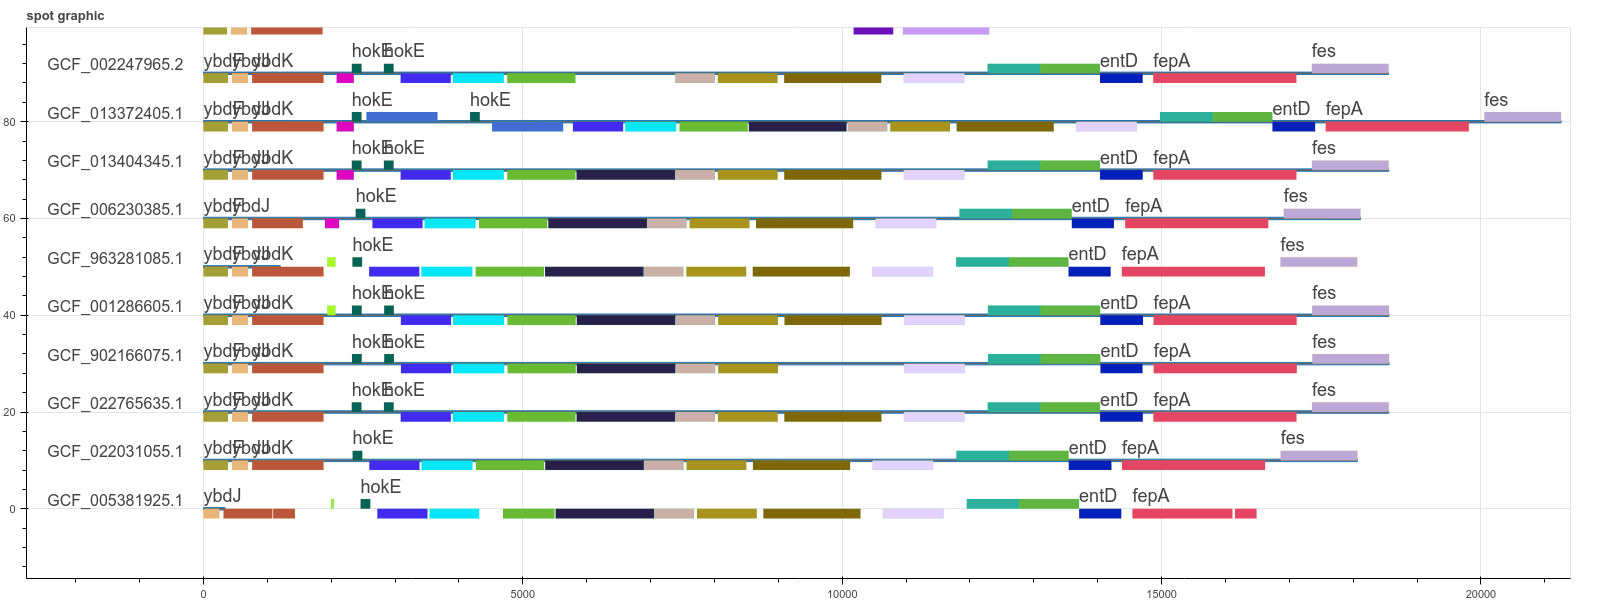
\includegraphics[width=0.6\textheight, angle=-90]{images/spot_181_fam.png}}
    \caption[Visualisation du spot 181 dans les génomes de \textit{E. coli}]{\textbf{Visualisation du spot 181 dans les génomes de \textit{E. coli}.} Les gènes sont représentés par des rectangles. (a) La couleur des gènes représente leur appartenance à un module. Les rectangles rouges indiquent que la famille correspondante appartient au module 752. La partition à laquelle le gène appartient est indiqué par la couleur du contour du rectangle : orange pour \textit{persistent}, vert pour le \textit{shell}. (b) La couleur des gènes représente la famille à laquelle appartient le gène.} 
    \label{fig:spot_apiose}
\end{figure}

L’identification du contexte génomique de la voie de dégradation du D-Apiose dans le spot 181 du pangénome de \textit{E. coli} constitue un indice supplémentaire en faveur d’une acquisition récente par transfert horizontal au sein de certaines lignées de \textit{E. coli}.

\section{Identification et annotation de la voie de dégradation dans une nouvelle souche : BVN-ST131}

En juin 2024, une nouvelle souche du type ST131 a été isolée par Van Nieuwenhuyse \textit{et al.} (2024) \cite{van_nieuwenhuyse_phage-mediated_2024}. Les auteurs ont réussi à séquencer et à obtenir le génome complet de cette souche. Dans ce contexte, nous avons cherché à identifier la présence de la voie alternative de dégradation du D-apiose au sein de cette souche et à l'associer au spot et au module précédemment détectés.

Pour ce faire, nous avons projeté le pangénome de \textit{E. coli} sur le génome de la souche BVN-ST131 (\autoref{fig:ProkseeApiose_complet}). Nous avons ensuite recherché la présence du \textbf{spot 181} et du \textbf{module 752}, lesquels sont associés au contexte dans le pangénome. L'exploration via la carte Proksee \cite{grant_proksee_2023} a permis d'identifier une région génomique présentant le spot et le module (\autoref{fig:ProkseeApiose_zoom}).

À partir de l'outil Proksee, nous avons procédé à l'alignement des protéines de la voie alternative de dégradation avec le génome de la souche, en utilisant BLAST \cite{altschul_basic_1990}, afin d'associer chaque gène identifié à une fonction spécifique (cercle externe en vert). Cette analyse a confirmé la présence de la voie alternative, incluant les 2 oxydoréductases. Par ailleurs, une annotation complémentaire des gènes restants a été réalisée à l'aide de Bakta \cite{schwengers_bakta_2021}, également via Proksee, ce qui a permis de retrouver les annotations précédemment identifiées dans le spot 181 (\textit{ABC transporter}, régulateur de transcription\dots).

L'identification de cette voie de dégradation dans une nouvelle souche du type ST131 confirme sa conservation au sein de ce groupe. Ces résultats vont dans le sens d'un rôle fonctionnel important dans l'adaptation et le métabolisme de ces souches, justifiant ainsi des investigations supplémentaires sur son impact physiologique et évolutif.

\begin{figure}[htbp] 
    \centering
    \subfloat[Génome circulaire de la souche BVN-ST131 de \textit{E. coli} ST131]{
        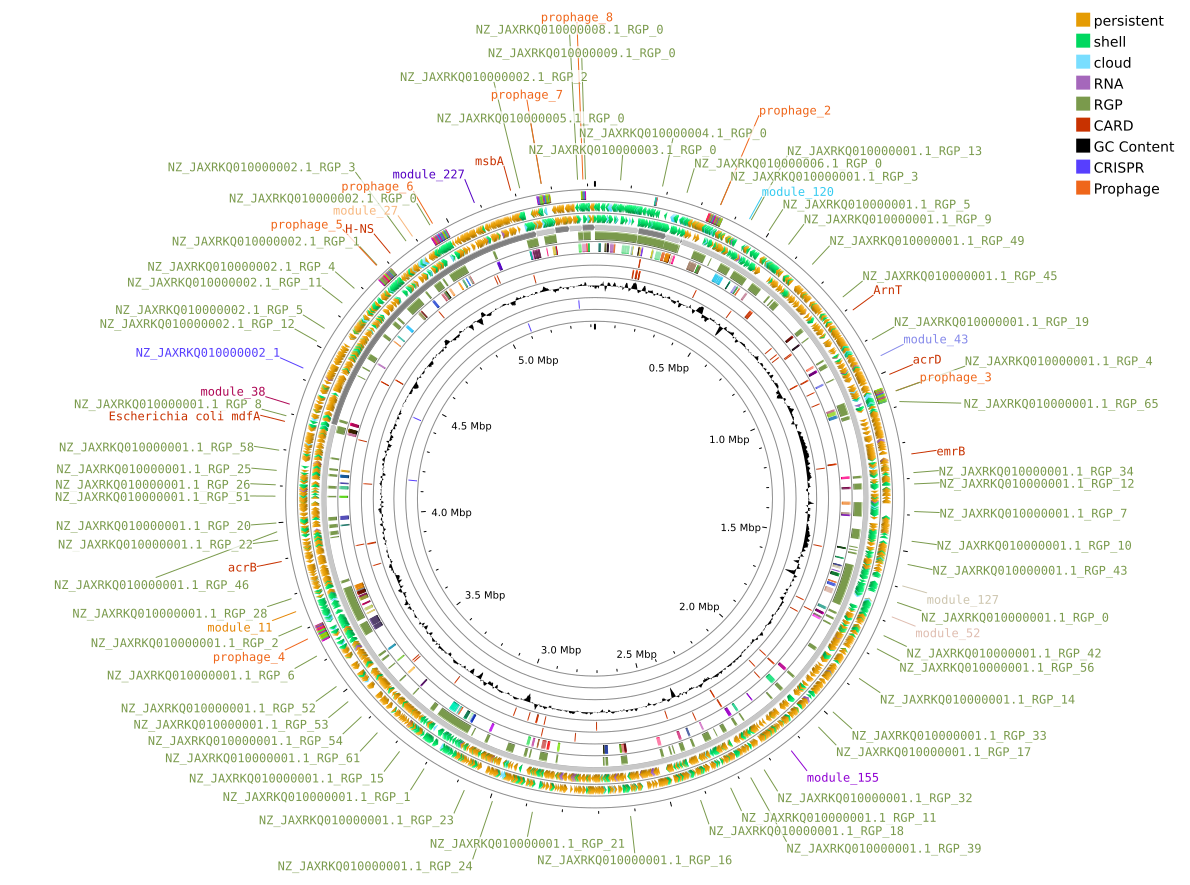
\includegraphics[width=.9\textwidth]{images/proksee_ST131.png}
        \label{fig:ProkseeApiose_complet}
        }
        
        \vspace{1cm} % Espace entre les deux images
        
        \subfloat[Spot 181 dans la souche BVN-ST131 de \textit{E. coli} ST131]{
        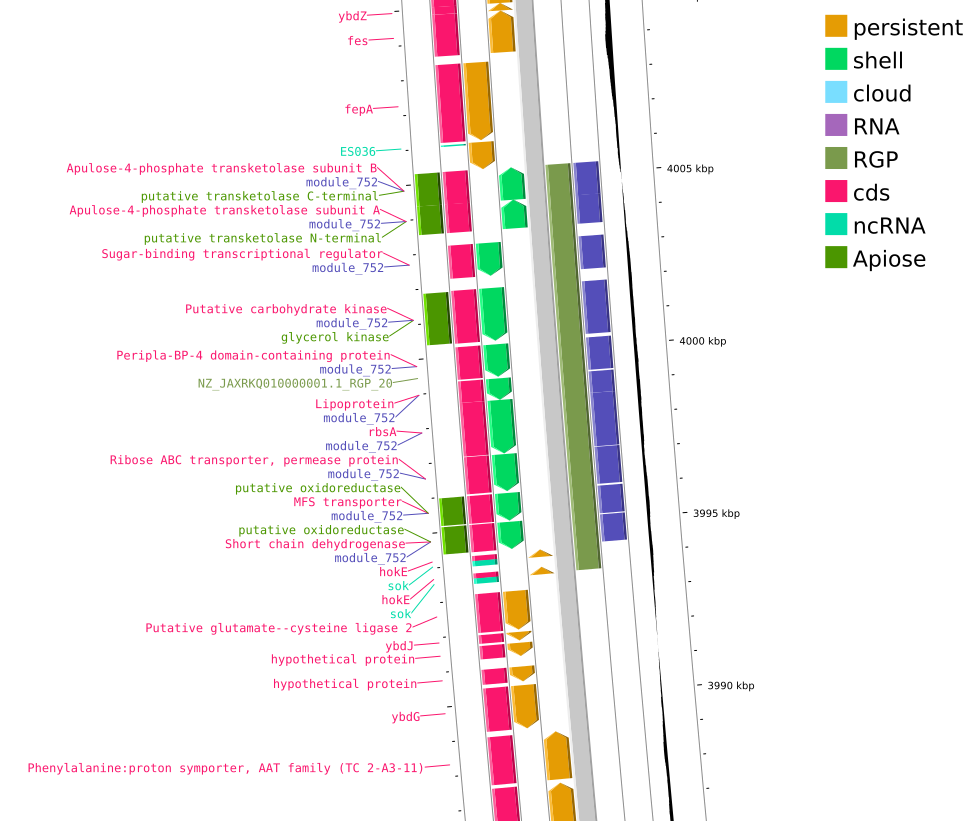
\includegraphics[height=.45\textheight]{images/proksee_apiose_ST131.png}
        \label{fig:ProkseeApiose_zoom}
        }
    \caption[Projection du pangénome de \textit{E. coli} sur le génome de la souche BVN-ST131]{\textbf{Projection du pangénome de \textit{E. coli} sur le génome de la souche BVN-ST131.} (a) } 
    \label{fig:ProkseeApiose}
\end{figure}

Afin de compléter notre analyse, nous avons utilisé les outils CARD \cite{alcock_card_2023} et Phigaro \cite{starikova_phigaro_2020} afin d’identifier respectivement les gènes de résistance aux antibiotiques et les régions prophages présentes dans le génome de la souche étudiée.

L’analyse a révélé la présence d’une RGP associée au gène \textit{mdtM}, conférant une résistance aux fluoroquinolones. Cette RGP a été retrouvée dans le \textbf{spot 99}, une région présente dans 1351 génomes, soit 67 \% du pangénome, ce qui suggère qu’il s’agit d’un hotspot d’insertion. Par ailleurs, une seconde RGP, d’une taille de 88 kpb, a été identifiée. Celle-ci contient 11 gènes de résistance à divers antibiotiques : les diaminopyrimidines, les sulfamides, les aminoglycosides, les macrolides et les tétracyclines. Bien que cette RGP ne soit pas associée à un spot, les familles correspondantes aux gènes de résistance se retrouvent dans les \textbf{modules 104} et \textbf{275}, détectés respectivement dans 645 et 252 génomes. De plus, une région prophage, colocalisée avec ces deux modules, a été identifiée et caractérisée par la présence de gènes codant des intégrases et des endonucléases.

Ces résultats mettent en évidence l’intérêt de l'identification des RGP et des régions prophages dans l'étude de la dispersion des gènes de résistance aux antibiotiques au sein du pangénome de \textit{E. coli}. L’association de ces éléments génétiques mobiles à des hotspots d’insertion et à des modules spécifiques suggère un rôle clé dans l’évolution et l’adaptation de ces souches, justifiant ainsi des analyses complémentaires sur leur impact fonctionnel et épidémiologique.